\documentclass[a4paper,12pt,oneside,openany,table,xcdraw]{article}

\usepackage{setspace}
\usepackage{multirow}
\usepackage{hyperref}
\usepackage{caption}
\usepackage{indentfirst}

\usepackage[brazilian]{babel}
\usepackage[utf8x]{inputenc}
\usepackage{amsmath, graphicx, enumerate}
\usepackage{float, verbatim}
\usepackage[colorinlistoftodos]{todonotes}
\usepackage{makeidx} % Para o sumário
\usepackage{geometry}

\geometry{a4paper, hmargin={3cm, 3cm}, vmargin={3cm, 2cm} }
\setlength{\parindent}{1.0cm}

\begin{document}
\newcommand{\thedepartment}{Faculdade de Engenharia Elétrica}
\newcommand{\thecourse}{FEELT}
\newcommand{\thetitle}{TENSÃO E CORRENTE DE CURTO-CIRCUITO EM REGULADOR DE TENSÃO SENOIDAL}
\newcommand{\thetype}{Relatório da Disciplina de Circuitos Elétricos II}
\newcommand{\theproftitle}{Bacharel em Engenharia Elétrica}
\newcommand{\thestudent}{Lesly Viviane Montúfar Berrios\\
\centering11811ETE001}
\newcommand{\theadvisor}{Prof. Wellington Maycon Santos Bernardes}
\newcommand{\thecity}{Uberlândia}

\thispagestyle{empty}\newcommand*{\themonth}{\ifthenelse{\the\month < 2}{Janeiro }
                  {\ifthenelse{\the\month < 3}{Fevereiro }
                  {\ifthenelse{\the\month < 4}{Março }
                  {\ifthenelse{\the\month < 5}{Abril }
                  {\ifthenelse{\the\month < 6}{Maio }
                  {\ifthenelse{\the\month < 7}{Junho }
                  {\ifthenelse{\the\month < 8}{Julho }
                  {\ifthenelse{\the\month < 9}{Agosto }
                  {\ifthenelse{\the\month < 10}{Setembro }
                  {\ifthenelse{\the\month < 11}{Outubro }
                  {\ifthenelse{\the\month < 12}{Novembro }{Dezembro }}}}}}}}}}}}
                  
\begin{titlepage}
\begin{center}

	\vspace{-0.5cm}

  \begin{figure}[hbt!]
		\begin{center}
		   
\includegraphics[width=2.8cm]{ufu-logo.png}
		\end{center}
	\end{figure}
 	%\vspace{-4cm}

%\begin{doublespacing}

  \Large{\textbf{Universidade Federal de Uberlândia}}\\
  \large{\thedepartment}\\
  \large{\thecourse}\\


\vspace{5.8cm}
  \par
  \large\textbf{\thetitle}
\vspace{5.8cm} 

%\end{doublespacing}
  \par
  \thetype\\
  por\\
  %\hspace{2cm}\large{}\\

\vspace{0.8cm}
\par
  \normalsize{\thestudent}\\ [2cm]
  \theadvisor

\par\vfill
  \thecity, \themonth / \the\year

\end{center}

\end{titlepage}

%% Comeca o documento !

\onehalfspacing
\tableofcontents % sumário
\newpage

\section{Objetivos} % 2,5%
Montar um circuito sob curto circuito, energizá-lo com tensão alternada senoidal e realizar medições usando equipamentos analógicos e digitais. Mostrar a importância de excursionar com cautela o regulador de tensão para identificação de curto-circuito nos primeiros instantes. Efetuar cálculos numéricos confrontando os resultados teóricos com aqueles obtidos experimentalmente.

\section{Introdução teórica} % 5%
O curto circuito ocorre quando não há carga conectada ao sistema, no entanto, em um sistema real, os fios condutores possuem certa resistência, mesmo que pequena. Sob essas circunstâncias, tem-se elevada potência passando pelo fio condutor, que pode não suportar e danificar o equipamento. 

\subsection{Potência em circuitos trifásicos}
Num circuito trifásico (estrela equilibrado), a potência total é dada por $P_{T}=3P_{F}$. A corrente de cada fase do circuito é igual a corrente de linha do alimentador e tensão de fase do alimentador é a tensão de linha ($E_{L}$ - Neutro-Fase) dividida por $\sqrt{3}$ \cite{irwin}. Assim a potência total será descrita como na Equação (\ref{potencia}).
\begin{equation*}
P_{T}=3\cdot \dfrac{E_{L}}{\sqrt{3}} I_{L}
\end{equation*}
\begin{equation}\label{potencia}
P_{T}=\sqrt{3}\cdot E_{L} I_{L}
\end{equation}

\section{Preparação}
\subsection{Materiais e ferramentas} % 2,5%
\begin{enumerate}[1 -]
\item \emph{\textbf{Fonte:}}
Alimentará todo o circuito.

\item \emph{\textbf{Regulador de tensão (Varivolt):}}
Também chamado de autotransformador, permitirá obter o valor desejado de corrente a partir da regulagem correta da tensão fornecida pela fonte.

\item \emph{\textbf{Conectores:}}
Para as conexões no circuito foi utilizado majoritariamente cabos banana-banana.

\item \emph{\textbf{Multímetros Digitais Minipa ET-2507A:}}
Foram utilizados 2, para medição da corrente e tensão do circuito em curto.

\item \emph{\textbf{Amperímetro analógico AC:}}
Instrumento utilizado para acompanhar visualmente o aumento da corrente.
\end{enumerate}

\subsection{Montagem} % 2,5%
\noindent\textbf{a.} Verifique se o interruptor está na posição desligada (\textit{OFF}).\\
\textbf{b.} Certifique que o regulador de tensão, também conhecido como \textit{varivolt}, está desligado ou com tensão mínima do lado secundário.\\
\textbf{c.} Alimente o lado primário do \textit{varivolt} usando a rede da CEMIG. Com um multímetro digital, anote o valor da tensão \textit{rms} em A’’N (Figura \ref{fig1}). Neste experimento obteu-se $V_{rms}=0,9V$.\\
\begin{figure}[H]
\centering
\captionsetup{font=scriptsize}
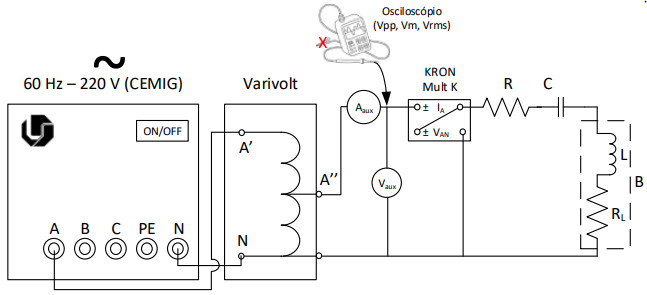
\includegraphics[width=14.5cm]{fig1}
\caption{Montagem experimental - parte 1.}
\label{fig1}
\end{figure}
\noindent\textbf{d.} Desligue a bancada por completo.\\
\textbf{e.} Sabendo que esse regulador de tensão trifásico é do modelo TSGC2-6, com potência nominal de 6 KVA, tensão de entrada nominal de 380 V e tensão de saída variável entre 0 e 430 V, calcule a corrente nominal de saída ($I_n$) desse equipamento. Utilizando-se a Equação (\ref{potencia}), determinou-se $I_{n}=\dfrac{P}{\sqrt{3}E_L}=\dfrac{6000}{\sqrt{3}430}=8,0561A$.\\
\textbf{f.} Calcule $I_{cc_max} = 75\%$ de $I_n$. Esse será o valor máximo de curto-circuito a ser utilizado nesse experimento por questões de segurança. $I_{cc_max}=0,75\cdot 8,0561A=6,0420A$.\\
\textbf{g.} Complete a ligação conforme a Figura \ref{fig2}. \\
\begin{figure}[H]
\centering
\captionsetup{font=scriptsize}
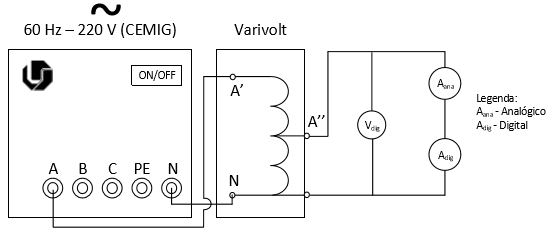
\includegraphics[width=14.5cm]{fig2}
\caption{Montagem experimental - parte 2.}
\label{fig2}
\end{figure}
\noindent\textbf{h.} NÃO ENERGIZE o circuito sem a autorização do professor para as próximas etapas. Neste momento, é fundamental chamá-lo para verificação passo-a-passo. \\
\textbf{i.} Ajuste e ligue os medidores digitais, ligue a bancada. Preenchendo a tabela abaixo com seis valores espaçados, aumente BEM VAGAROSAMENTE a tensão no \textit{varivolt} até as correntes de curto circuito nos amperímetros indicar aproximadamente $I_{cc_max}$. Não deixe os medidores ligados por mais de 2 minutos para evitar aquecimento por efeito \textit{Joule}.  \\

\begin{table}[H]\scriptsize
\centering
\def\arraystretch{1.35}
\captionsetup{font=scriptsize}
\captionof{table}{Dados experimentais de tensão e corrente.} \label{tab2}
\begin{tabular}{|c|c|}
\hline
$I_{CC}$ & $V_{CC}$ \\ \hline
1,300    & 0,260    \\ \hline
1,500    & 0,320    \\ \hline
1,923    & 0,488    \\ \hline
2,199    & 0,498    \\ \hline
3,012    & 0,612    \\ \hline
4,36     & 0,881    \\ \hline
5,054    & 1,029    \\ \hline
5,190    & 1,054    \\ \hline
5,959    & 1,208    \\ \hline
\end{tabular}
\end{table}

A utilização de dois amperímetros é por questões de redundância, apenas. O amperímetro analógico é adequado para visualizar a velocidade da variação da corrente, enquanto no digital, o resultado é apresentado com maior quantidade de casas decimais. Todavia, o amperímetro digital apresenta uma barra gráfica analógica para proporcionar essa indicação visual. 

\noindent\textbf{j.} Retorne a tensão no varivolt para o valor mínimo de tensão, desligue a bancada e os medidores digitais.\\

\section{Análise sobre segurança} % 2,5%
Os óculos de segurança são Equipamentos de Proteção Individual (EPIs) e são utilizados para a proteção da área ao redor dos olhos contra qualquer tipo de detrito estranho, que possa causar irritação ou ferimentos. Também protegem contra faíscas, respingos de produtos químicos, detritos, poeira, radiação e etc \cite{safe}.
É importante a utilização desse equipamento durante os experimentos a fim de evitar qualquer dano, além de preparar o profissional para o manejo correto e seguro de qualquer equipamento.
Além disso, foi de extrema importância a presença do professor ou técnico na verificação da montagem do circuito antes de energizá-lo. Assim, reduziu-se riscos de curtos-circuitos ou sobrecarga na rede.

\section{Cálculos, análise dos resultados e questões} % (quando houver) (70%)
\begin{enumerate}[1)]
\item Encontre o erro percentual da corrente nominal de saída calculado ($I_n$) e o valor informado na placa ou manual técnico do equipamento.\\
O valor informado na placa do equipamento é de $8V$. Assim, há um erro percentual de $-0,7\%$.

\item Trace um gráfico $f(V_{cc}\times I_{cc})$. Estime o valor de $V_{cc}$ quando $Icc=100\%$ de $I_n$ por meio de interpolação ou método dos mínimos quadrados.\\
Pelo gráfico da Figura \ref{graph}, tem-se a reta de regressão linear dada por $y=0,1243x+0,0840$. Para $x=8,0561$ tem-se $y=1,0854$, que corresponde à tensão $V_{cc}=1,0854$ para $Icc=100\%$ de $I_n$. Note que é um valor aproximado.

\begin{figure}[H]
\centering
\captionsetup{font=scriptsize}
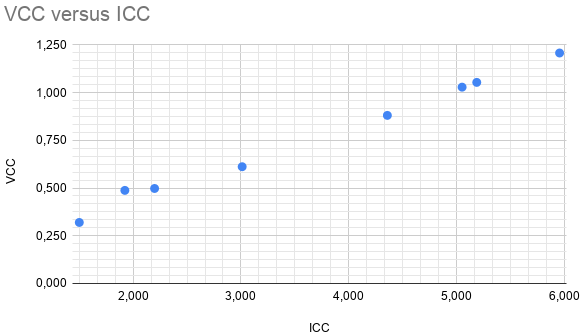
\includegraphics[width=14.5cm]{graph}
\caption{Gráfico $f(V_{cc}\times I_{cc})$ gerado em excel.}
\label{graph}
\end{figure}

\item Determine o valor da impedância em condição de curto-circuito - $Z_{cc}$.\\
Pela relação $V=Z\cdot I$, a impedância do circuito será o valor de inclinação da reta de regressão linear, $Z_{cc}=0,1243\Omega$.

\item Estime o valor de $V_{cc}$ para $110\%$ e $150\%$ de $I_n$. Diante disso, explique a importância de observar em primeiro lugar o amperímetro nos experimentos da disciplina.\\
Utilizando-se a equação da reta de regressão linear $y=0,1243x+0,0840$, tem-se que para $110\%$ e $150\%$ de $I_n$, ou seja, $x_1=8,0561\cdot1,1$ e $x_2=8,0561\cdot1,5$, a tensão $V_{cc}$ do sistema será, respectivamente, $V_{cc, 1}=1,1855 V$ e $V_{cc, 2}=1,5861 V$. Verfica-se que para pequenas variações na tensão há notável aumento da corrente de curto, o que pode danificar o equipamento se não manejado de forma correta e segura. 

\item Por que o medidor eletrônico \emph{KRON Mult K} não pode ser utilizado nas condições apresentadas desse experimento?\\
Não pode ser utilizado uma vez que a corrente nominal de saída do equipamento é de $5V$ e como as condições do experimento exigem valores de corrente superior a esse, há perigo de danificar o equipamento.

\item Sabendo agora como o regulador de tensão TSGC2-6 se comporta diante de uma corrente de curto-circuito, qual(is) procedimentos você pode adotar ao ligar um circuito elétrico pela primeira vez? Essa aula pode ser aplicada em outros dispositivos? Se sim, qual(is)?\\
Verificar a variação da corrente antes de se aplicar uma tensão, com intuito de detectar uma possível situação de cuto circuito.
É possível aplicar os conhecimentos dessa aula para qualquer equipamento, pois qualquer equipamento tem uma corrente máxima que pode ser suportada.

\end{enumerate}
\section{Simulação computacional} % (10%);

\section{Conclusões} % (no mínimo 10 linhas) (5%);
Verfica-se que para pequenas variações na tensão há notável aumento da corrente de curto, o que pode danificar o equipamento se não manejado de forma correta e segura. Assim, é essencial verificar a variação da corrente antes de se aplicar uma tensão, com intuito de detectar uma possível situação de cuto circuito.

É possível aplicar os conhecimentos dessa aula para qualquer equipamento, pois qualquer equipamento tem uma corrente máxima que pode ser suportada. Neste experimento, o objetivo de efetuar cálculos numéricos confrontando os resultados teóricos com aqueles obtidos experimentalmente foi cumprimdo para a realização da tarefa de detectar experimentalmente o que acontece num curto.

\newpage
\begin{thebibliography}{9} 
% Introdução
\bibitem{irwin}
    J. D. Irwin,
    “Análise de Circuitos Em Engenharia”, Pearson, $4^a$ Ed., 2000.

\bibitem{boylestad}
    R. L. Boylestad,
    “Introdução À Análise de Circuitos”, Pearson, $10^a$ Ed., 2004.

\bibitem{safe}
    SafetyTrabi,
    “Óculos de segurança: Saiba quando utilizar este EPI”, SafetyTrab, 2019.
 Disponível em:
 \url{https://www.safetytrab.com.br/blog/oculos-de-seguranca/}. Acesso em: ago. 2019.


\end{thebibliography}
\end{document}
